\chapter{Objetivos}\label{chap:objetivos}
Una vez explicado en el ámbito en el que se realiza este proyecto, en este capitulo explicaremos los objetivos que se han tratado de alcanzar y el método de trabajo que se ha seguido para lograrlo

\section{Objetivos del TFG}
El objetivo de este trabajo es dar soporte en la plataforma de \textit{Kibotics} \footnote{\url{https://kibotics.org/}} a un robot bastante popular para la robótica educativa como es el \textit{LEGO Ev3}, esto significa integrarlo de forma que se pueda programar dentro de la plataforma, y que también funcione para el robot real.\newline 
\textbf{Soporte Simulado}
\begin{itemize}
    \item Añadir una simulación 3D realista sabiendo que hay modelos de robots prediseñados por \textit{LEGO} de varios modelos de robots, al menos uno por cada tipo de sensor que pueda llevar. Y que tenga sentido físico dentro de la simulación.
        
    \item Añadir la infraestructura necesaria como \textit{drivers}, y funciones al \textit{Robot API} para que el robot se programable en cualquier lenguaje soportado por la plataforma, y funcione en el robot real
    
    \item Crear un conjunto de ejercicios para que haya un temario fácil de seguir por el estudiante, y con una curva de dificultad moderada
    
\end{itemize}
\textbf{Soporte Real}
\begin{itemize}
    \item Instalar una imagen de un sistema operativo en el \textit{Lego ev3} en este caso, una distribución basada en \textit{Debian Linux}.
    \item Instalar un servidor en el robot capaz de recibir mensajes con el código, y lo transforme en un archivo y lo ejecute dentro de la máquina.
    
\end{itemize}
\section{Metodología}
\label{sec:metodologia}

La metodología para completar el trabajo de fin de grado se puede dividir en diferentes fases que se iban repitiendo cada cierto tiempo, en cada una de ellas, semanalmente, tenia lugar una reunión con el tutor del trabajo para determinar los siguientes objetivos a cumplir y evaluar las tareas propuestas en anteriores sesiones. Esto ayuda mucho en proyectos como este, en constante desarrollo.\newline
Este proyecto se lleva a cabo con un equipo de trabajo, que se ocupa de la plataforma de \textit{Kibotics}, cada uno con sus labores y ocupaciones. Por lo tanto, es necesaria la comunicación y realimentación con el resto de integrantes. Para ello se utiliza la herramienta \textit{Slack}\footnote{\url{https://slack.com/}} en la que los desarrolladores están en contacto en todo momento, no solo para comunicar avances, si no también para ayudar en todo momento si surge algún contratiempo en el desarrollo.\newline
Para trabajar en local, con el repositorio original me hice \textit{git clone} de los repositorios que necesitaba, e iba trabajando sobre ellos, guardando los cambios en un repositorio creado solo para el trabajo de fin de grado \footnote{\url{https://github.com/RoboticsLabURJC/2020-tfg-daniel-pulido}} hasta que la funcionalidad estaba completa, que era cuando se subían al repositorio principal. Esta metodología, es el llamado modelo iterativo de desarrollo de software.



 \begin{figure}[H]
    \centering
    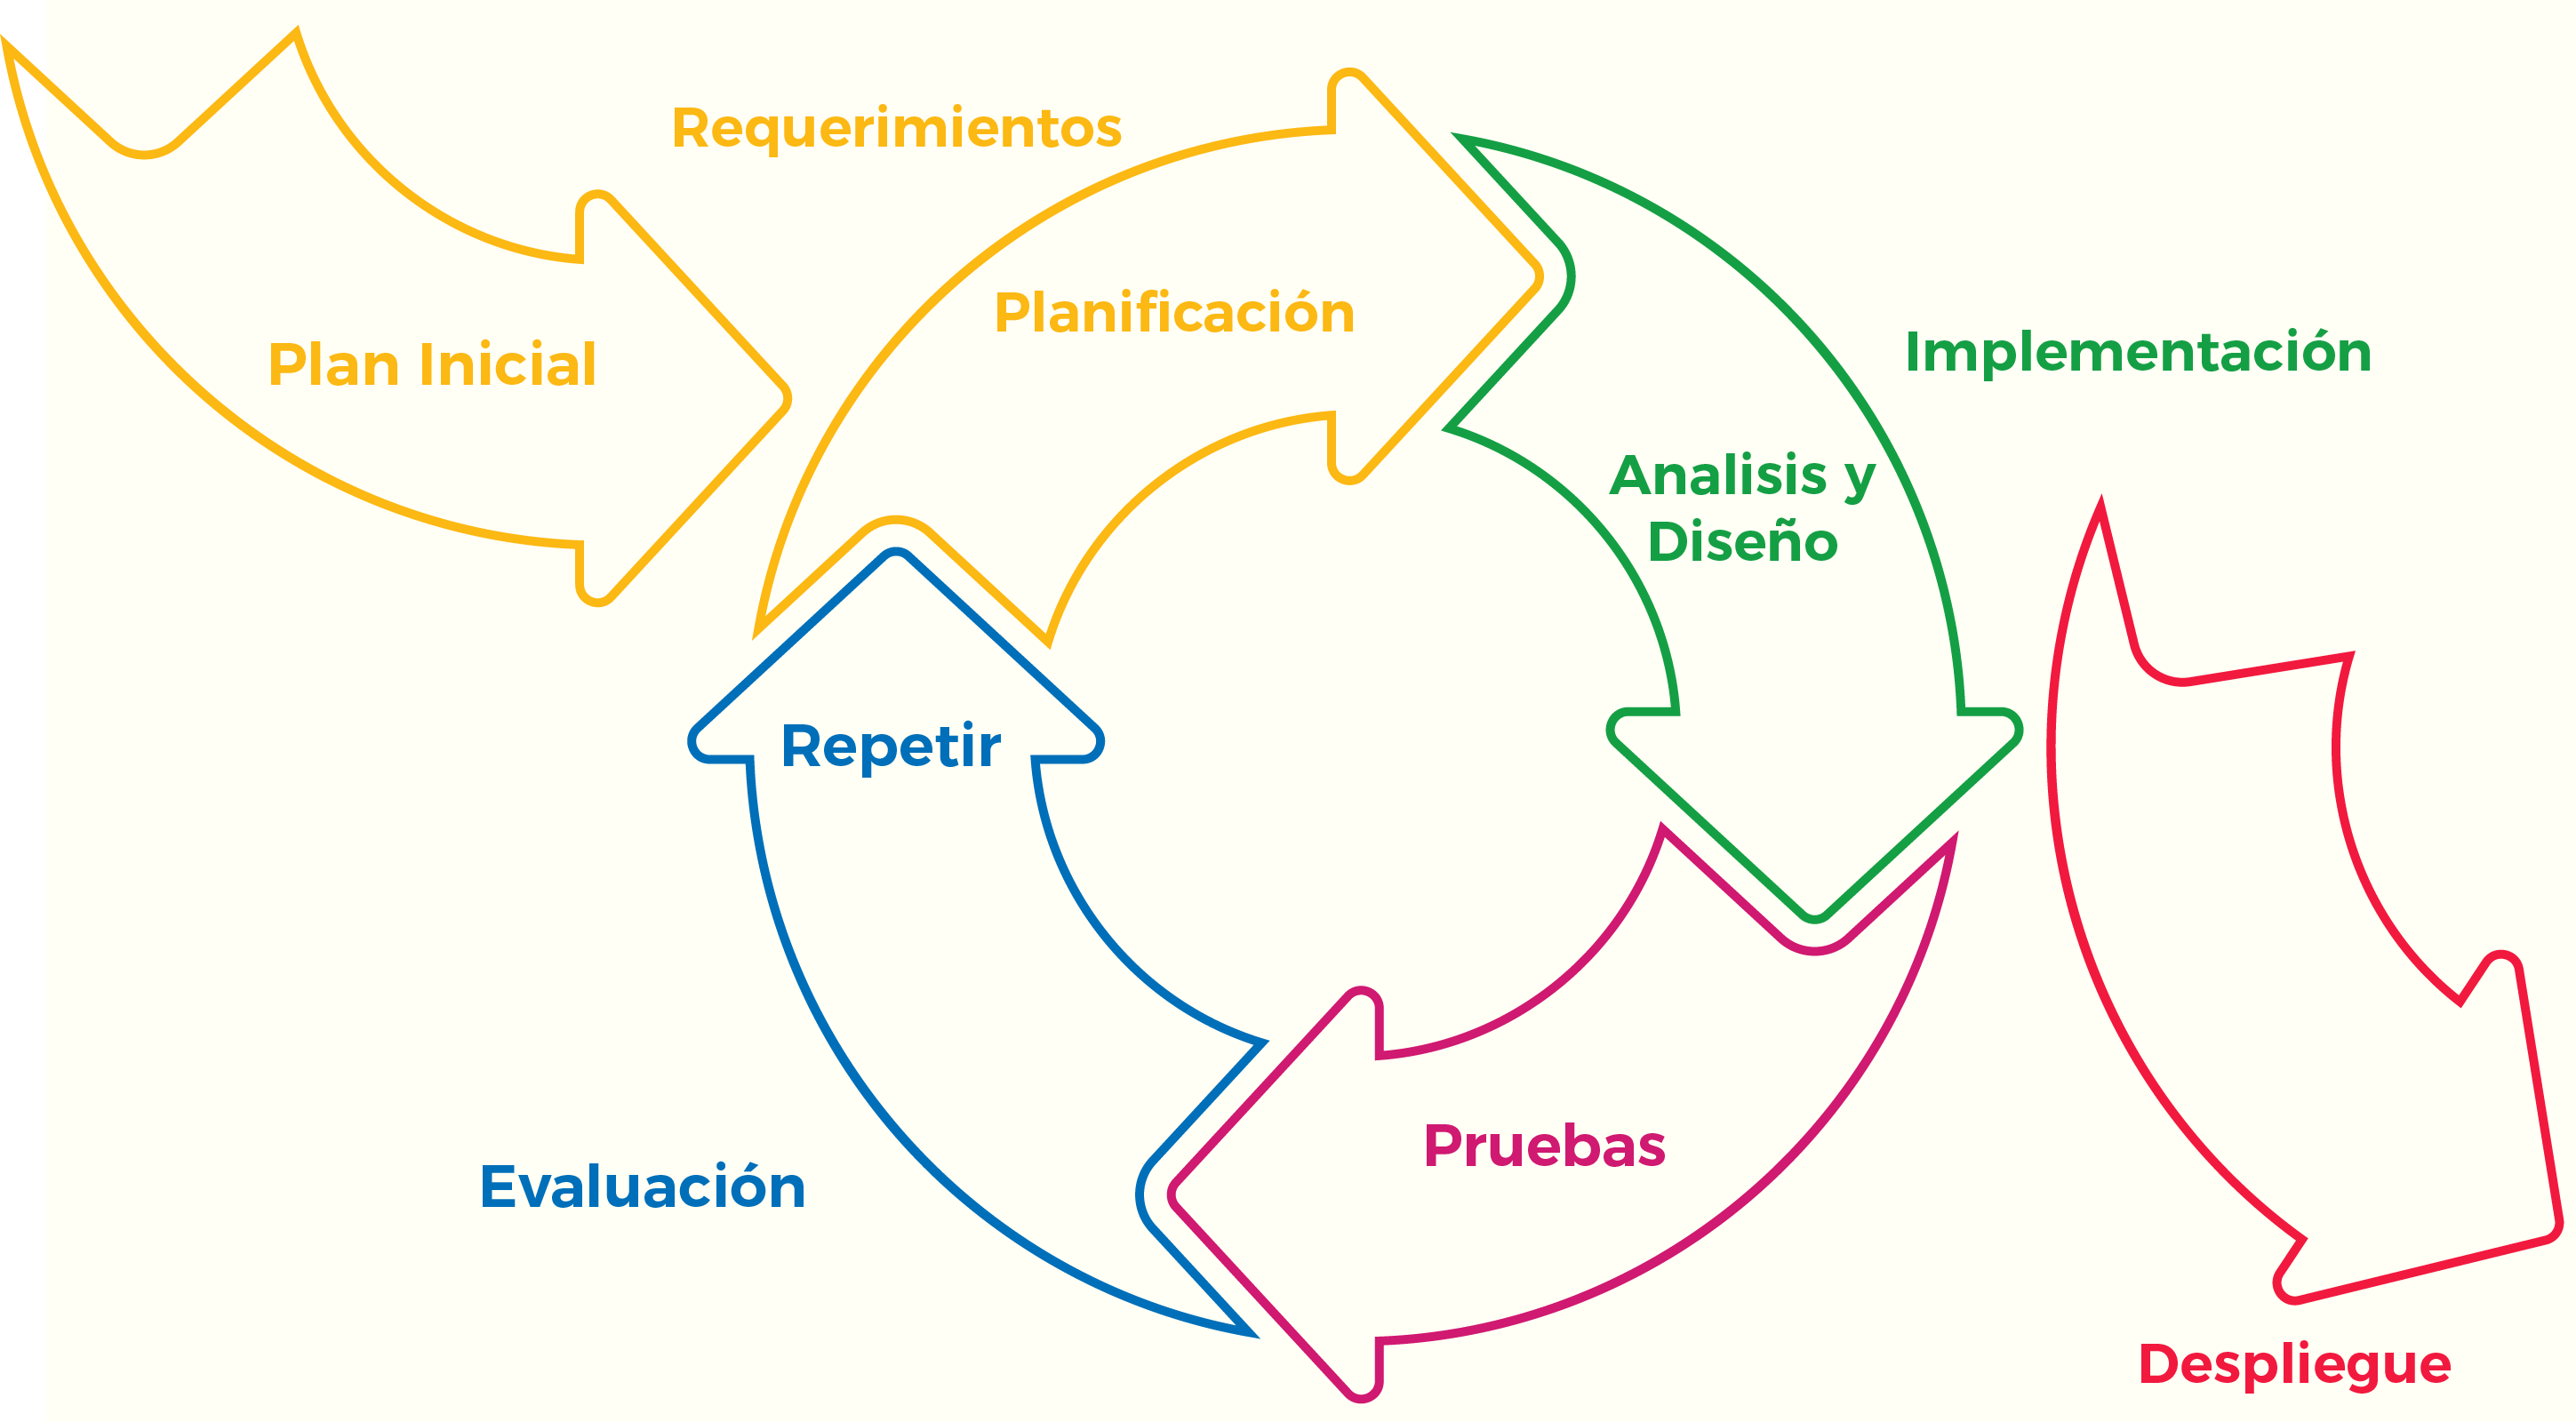
\includegraphics[width=0.9\textwidth]{img/metodoiterativo.png}
    \caption{Metodología de modelo iterativo} \label{fig:metodo}
\end{figure}

Cuando los cambios eran revisados por el tutor, se seguía una dinámica de \textit{Incidencia y parche} en el repositorio principal. Para ello se creaba una incidencia (\textit{issues}) con el tema que se iba a solucionar o añadir en la funcionalidad de la plataforma, y una vez resuelto en local y para cerrarla, se creaba una rama (\textit{branch}) creando parche (\textit{pull request}) para que un desarrollador principal de \textit{Kibotics}, lo aceptará y fusionará con la rama principal y así arreglar la incidencia. Esto se hace para registrar todos los cambios, y comprobarlos antes de que se trabaje directamente en el repositorio



\section{Requisitos}
\label{sec:requisitos}
Para completar la integración del robot \textbf{LEGO Ev3} se necesitan ciertos requisitos que cumplir:
\begin{itemize}
    \item Dentro del \textbf{LEGO Ev3} debe correr una distribución de \textit{Linux} , en este caso he optado por la imagen creada por \textit{ev3dev}, que es una distribución basada en el sistema operativo \textit{Debian Linux}, de la cual entrare en mas detalle en el Capitulo 5: \textit{Soporte Lego ev3 físico}.
    \item El resultado final debe ser lo más sencillo posible, no debe requerir configuraciones adicionales. Este software tiene que estar diseñado para estudiantes. 
\end{itemize}    

\section{Plan de trabajo}
\label{sec:plan}

El plan de trabajo a seguir para conseguir el objetivo se puede dividir en los siguientes pasos:
\begin{itemize}
    \item \textit{Paso 1}: Aterrizaje en \textit{Kibotics}. Lo primero que hay que hacer es familiarizarse con el entorno con el que se va a trabajar. \textit{Kibotics} es una plataforma web en la que entraremos mas en detalle en el siguiente capitulo 
    \item \textit{Paso 2}: Comienzo de la creación del robot simulado. Comenzaremos por la creación de varios modelos 3D para usarlos en el entorno simulado, son varios diferentes ya que lo original que tiene \textit{LEGO} es poder construir tu robot en base a la tarea que vaya a realizar, con las piezas que incluye el kit .
    \item \textit{Paso 3}: Desarrollo de las funciones y ejercicios dentro de la aplicación de \textit{Kibotics} para crear una dinámica de trabajo con el nuevo robot.
    \item \textit{Paso 4}: Dar soporte al robot real para poder programarlo en \textit{python} desde el exterior, y la instalación de un server para que pueda recibir código y ejecutarlo en local. 
    \item \textit{Paso 5}: Creación de los \textit{drivers} que hagan de traductor entre lo que creas en la plataforma, y lo que entiende el robot. 
\end{itemize}